\section{Nombre: Nexoxcho}  \label{per:nexoxcho}
\subsection{Descripción:}
Nexoxcho no posee una forma definida, su fisico depende de quien lo mire pues encarna los miedos más profundos de las personas.
\\
\par
En su encuentro contra Malinalli, Nexoxcho adopta la forma del Padre de ésta pero en un estado de corrupción y degradación espiritual. En esta forma el se muestra sin ojos, con las heridas de puñaladad altamente visibles y sin un corazón. De sus heridas brota un liquido negro que simula la corrupción en el alma. 
\\
\par
Nexoxcho es un dios callado y tímido. Al ser consciente de los daños que puede causarle a la psique de los Dioses, evita toparse con los demás por lo que es un dios bastante solitario. No acostumbra a luchar físicamente, el efecto que tienen sus poderes usualmente le garantiza la victoria contra cualquier enemigo.         
\subsection{Status:}
	\begin{itemize}
		\item Personaje no jugable.
		\item Enemigo jefe.
	\end{itemize}
\subsection{Imagen}
Ver figura \ref{fig:nexoxchoDiseno}
	\begin{figure}
					\centering
					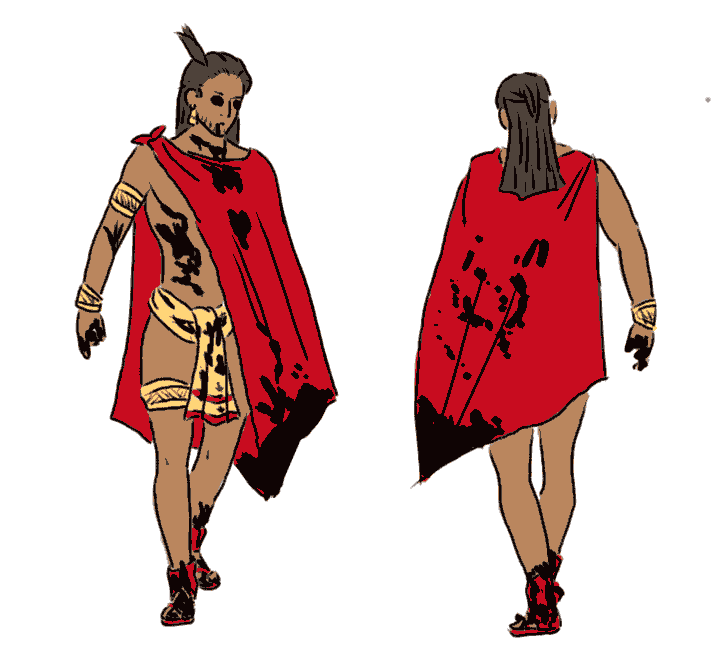
\includegraphics[height=0.3 \textheight]{Imagenes/nexoxcho}
					\caption{Concepto de diseño de Nexoxcho.}
					\label{fig:nexoxchoDiseno}
	\end{figure}
\subsection{Concepto:}
\begin{itemize}
	\item \textbf{Historia antes del juego:}
	Nexoxcho se ofrece de manera voluntaria a ser uno de los guardianes del Mictán durante los tiempos de restauriacion del orden luego de las rebeliones que se produjeron por la creación del quinto Sol. Pues consideraba que sus habilidades eran más útiles para los demás dioses en el Mictlan que en los trece cielos donde podía lastimar a alguien si querer.
	\item \textbf{Historia durante el juego:}
	Al ver que los demás guardianes eran derrotados sin mayor problema, Nexoxcho comprende que es su responsabilidad  absoluta frenar el avance de Xólotl.
	\item \textbf{Relaciones:}
	\begin{itemize}
		\item \textbf{Xólotl:} Nexoxcho considera a Xólotl como un ser mal agradecido e infantil. Desde su punto de vista Xólotl no tiene motivos para estar molesto (ver aparatado \ref{per:xolotl}). 
		\item \textbf{Nota:} Nexoxcho no puede relacionarse con los demás Dioses debido a sus poderes por lo que no goza de ningún vinculo con el resto. 
	\end{itemize}                     
\end{itemize}

\subsection{Encuentro:}
\begin{itemize}
	\item Su primera aparición es en la cinemática 9 (ver aparatado \ref{Cin:Cinematica09}).
	\item Como jefe, el juagdor se enfrenta a él en el octavo nivel del juego (ver aparatado \ref{Nivel:Niv08}).
\end{itemize}

\subsection{Habilidades:}
Nexoxcho puede ver los miedos reales de las personas y convertirlos en peligrosas ilusiones en donde atrapa a quien lo mire.  

\subsection{Armas:}
Sin armas.
\subsection{Ítems:}
Sin ítems.
\subsection{Bloques de animación}
\begin{itemize}
	\item Padre de Malinalli corrompido.
		\begin{itemize}
			\item Animación apuñalar.
			\item Animación caminar.
			\item Animación recibir daño.
			\item Animación morir.
		\end{itemize}
\end{itemize}